
The \ttjets process is the most dominant background for this analysis. Two types of 
\ttjets MC samples, one generated with MadGraph-MLM and other with $POWHEG$ are 
officially available. However, choice of \ttjets sample from these two depends on the
number of jets present in the final states. For high jet multiplicity, the MadGraph-MLM sample is 
not properly modeled. In this analysis, we require each event to have at least 4 jets so the
$POWHEG$ \ttjets sample is preferred over that from MadGraph-MLM. 

For the sake of comparison, \ttjets sample from both generator is analysed. The number 
of events after various selection cuts are shown in Figure~\ref{fig:MGvsPG} for \mujets and 
\ejets channels. For both channels, the number of events is exactly the same up to the 
relative isolation selection. After requiring the events to have $N_{jets} \geq 4$, the
\ttjets sample from both generator give different event yields. The data, MC agreement
after the kinematic fit selection is better with $POWHEG$ \ttjets sample as compared
to that from MadGraph-MLM. In view of this the $POWHEG$ \ttjets sample is used in this
analysis.  

\begin{figure}
    \centering
    \subfigure[With MadGraph-MLM \ttjets sample 
    \label{subfig:cutflow_mu_MG}]
    {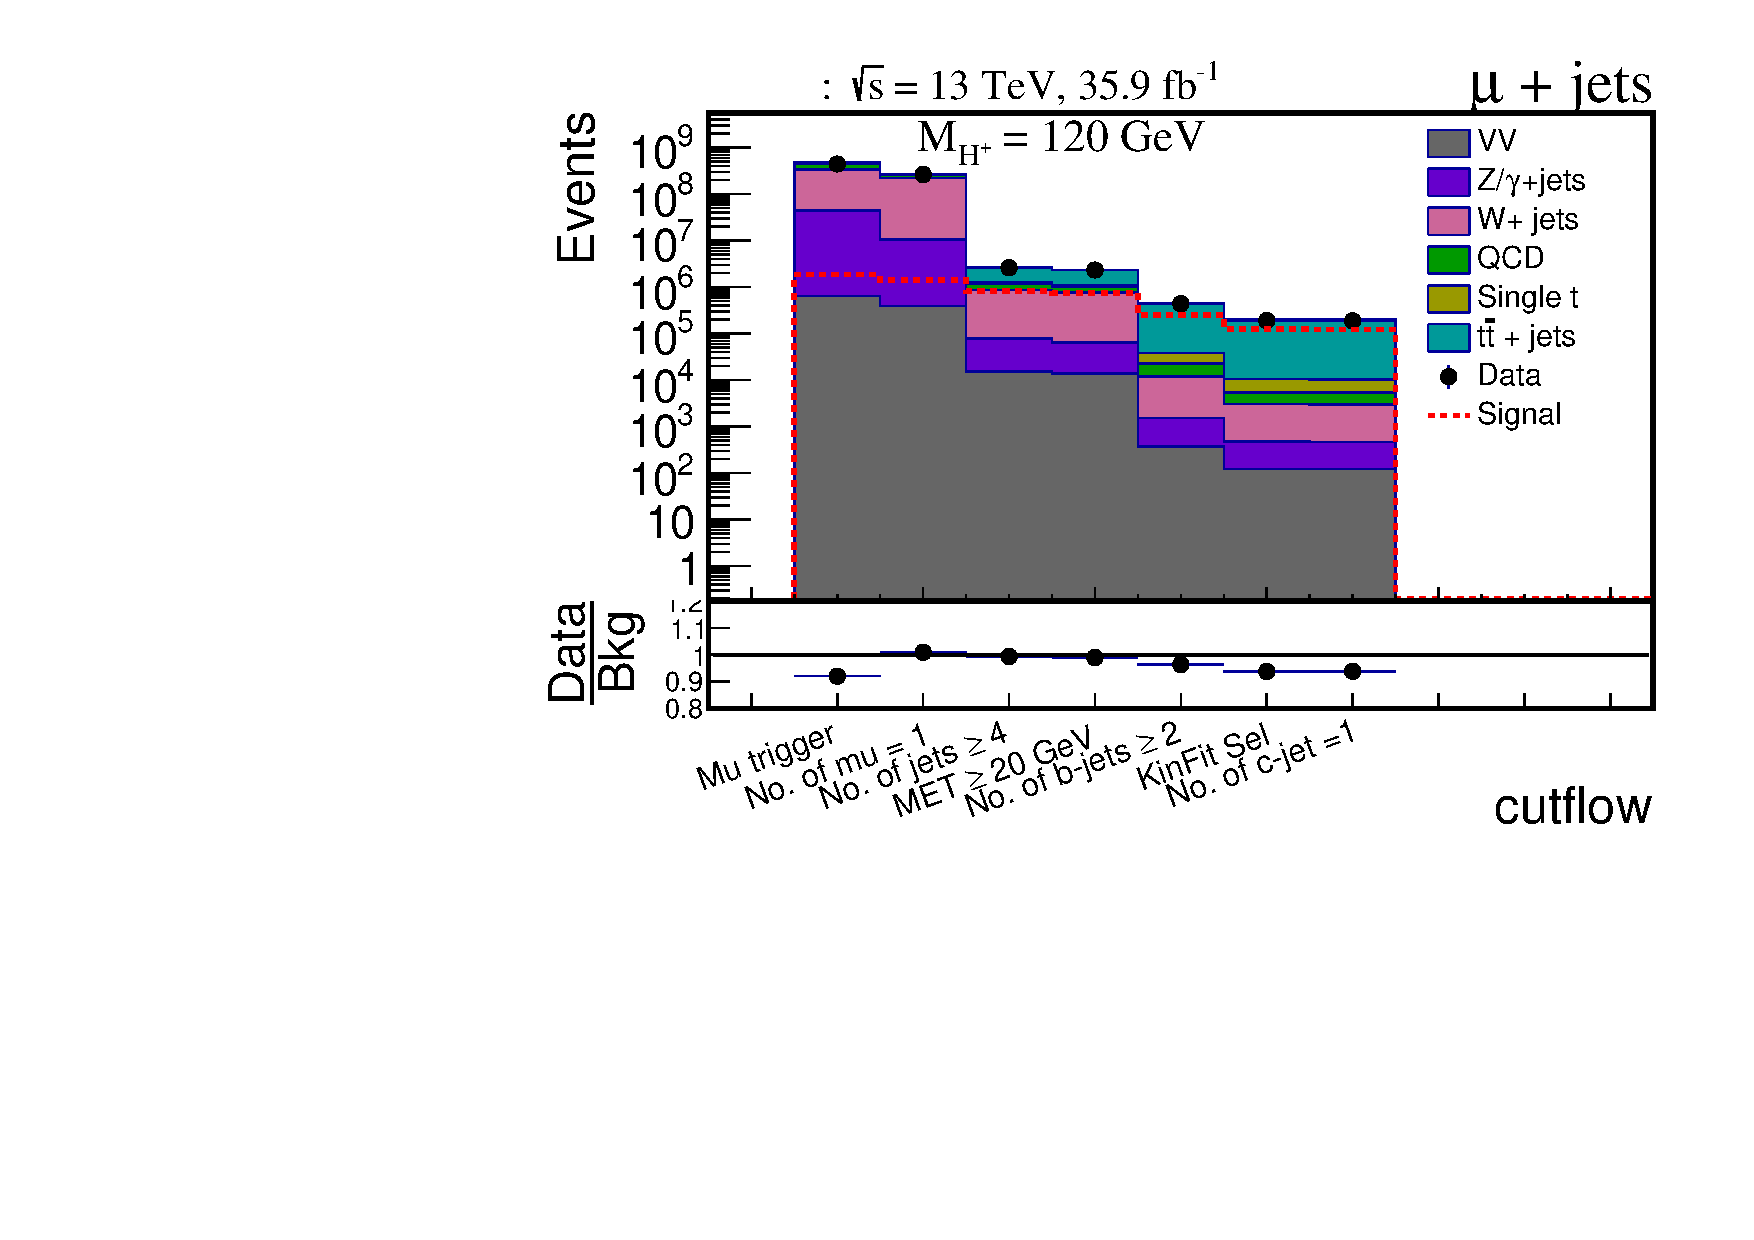
\includegraphics[width=0.45\linewidth]{Image/Muon/cutflow_mu_MG.pdf}}
    \subfigure[With MadGraph-MLM \ttjets sample 
    \label{subfig:cutflow_ele_MG}]
    {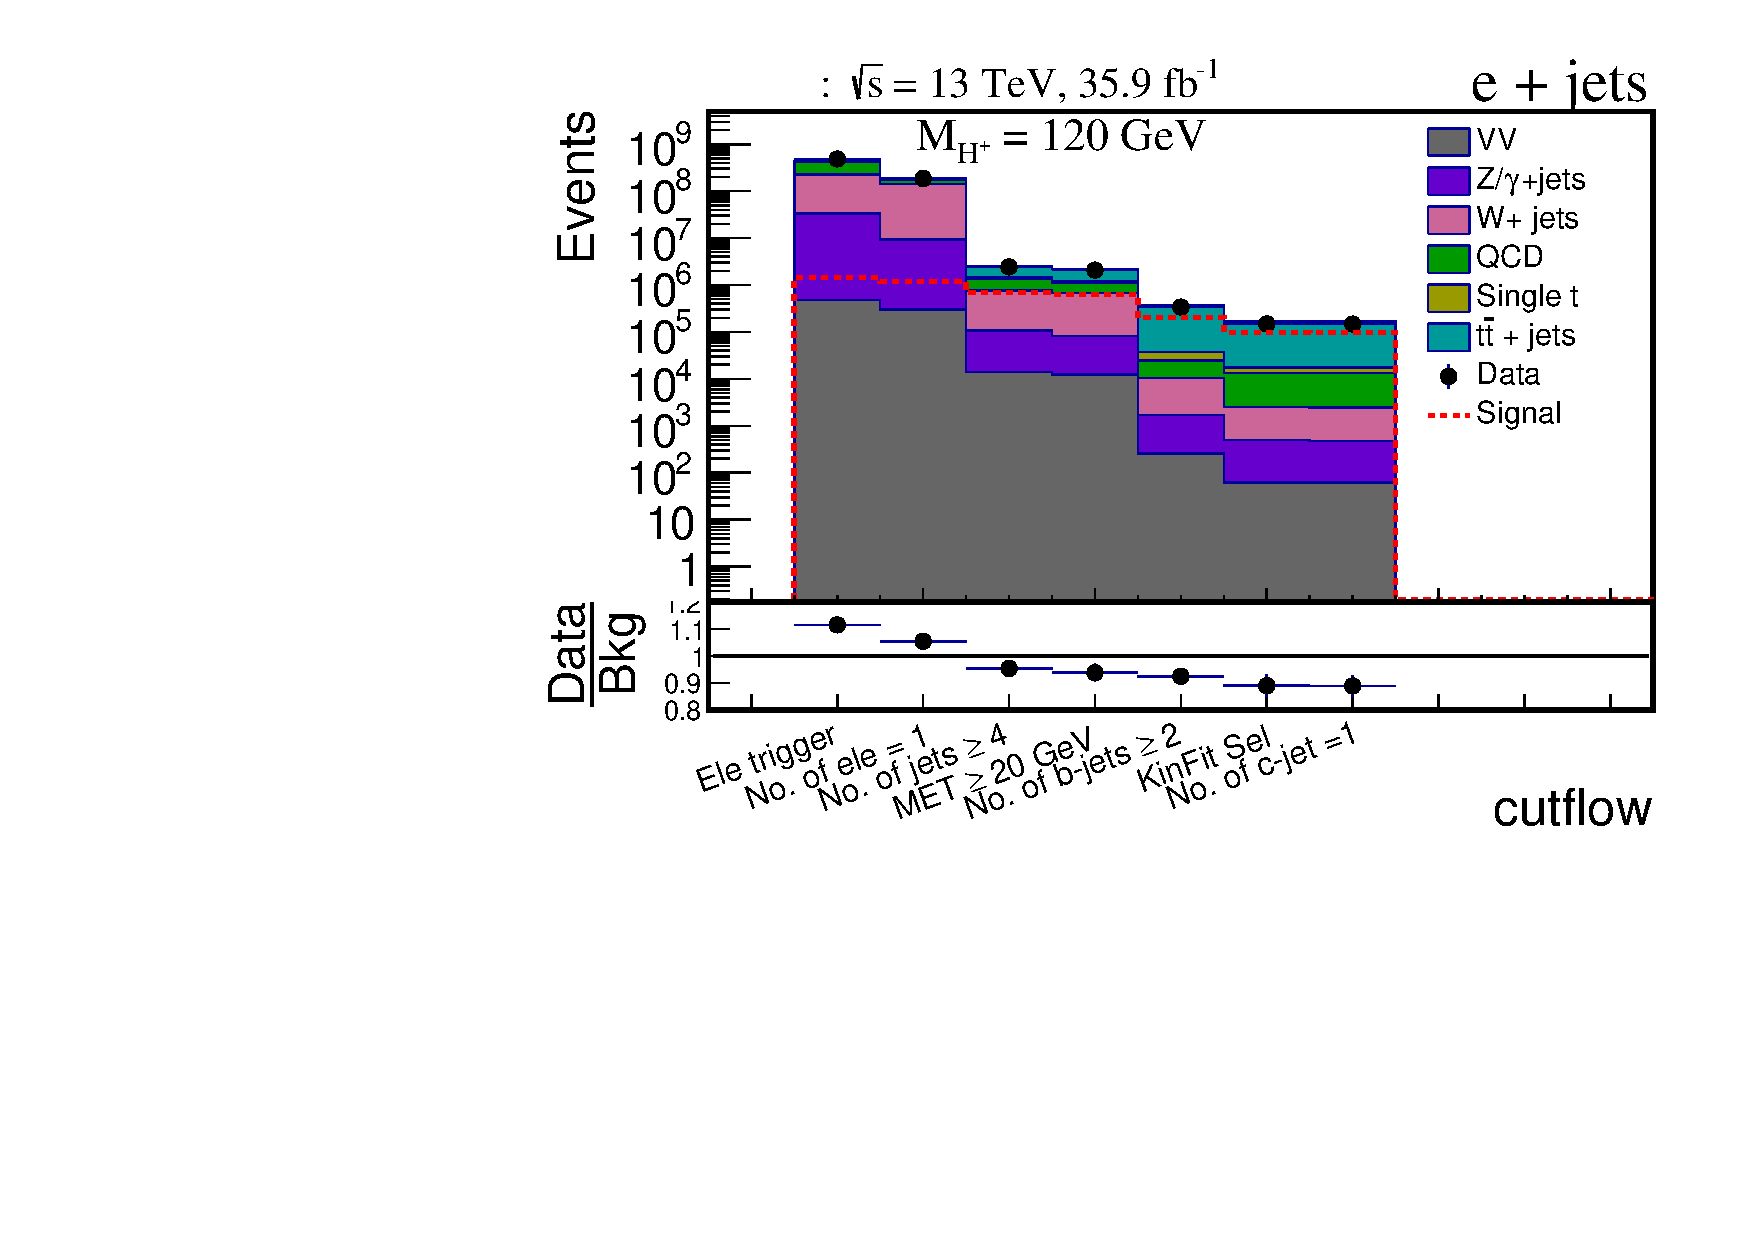
\includegraphics[width=0.45\linewidth]{Image/Electron/cutflow_ele_MG.pdf}}

    \vfil
    \subfigure[With $POWHEG$ \ttjets sample
    \label{subfig:cutflow_mu_PG}]
    {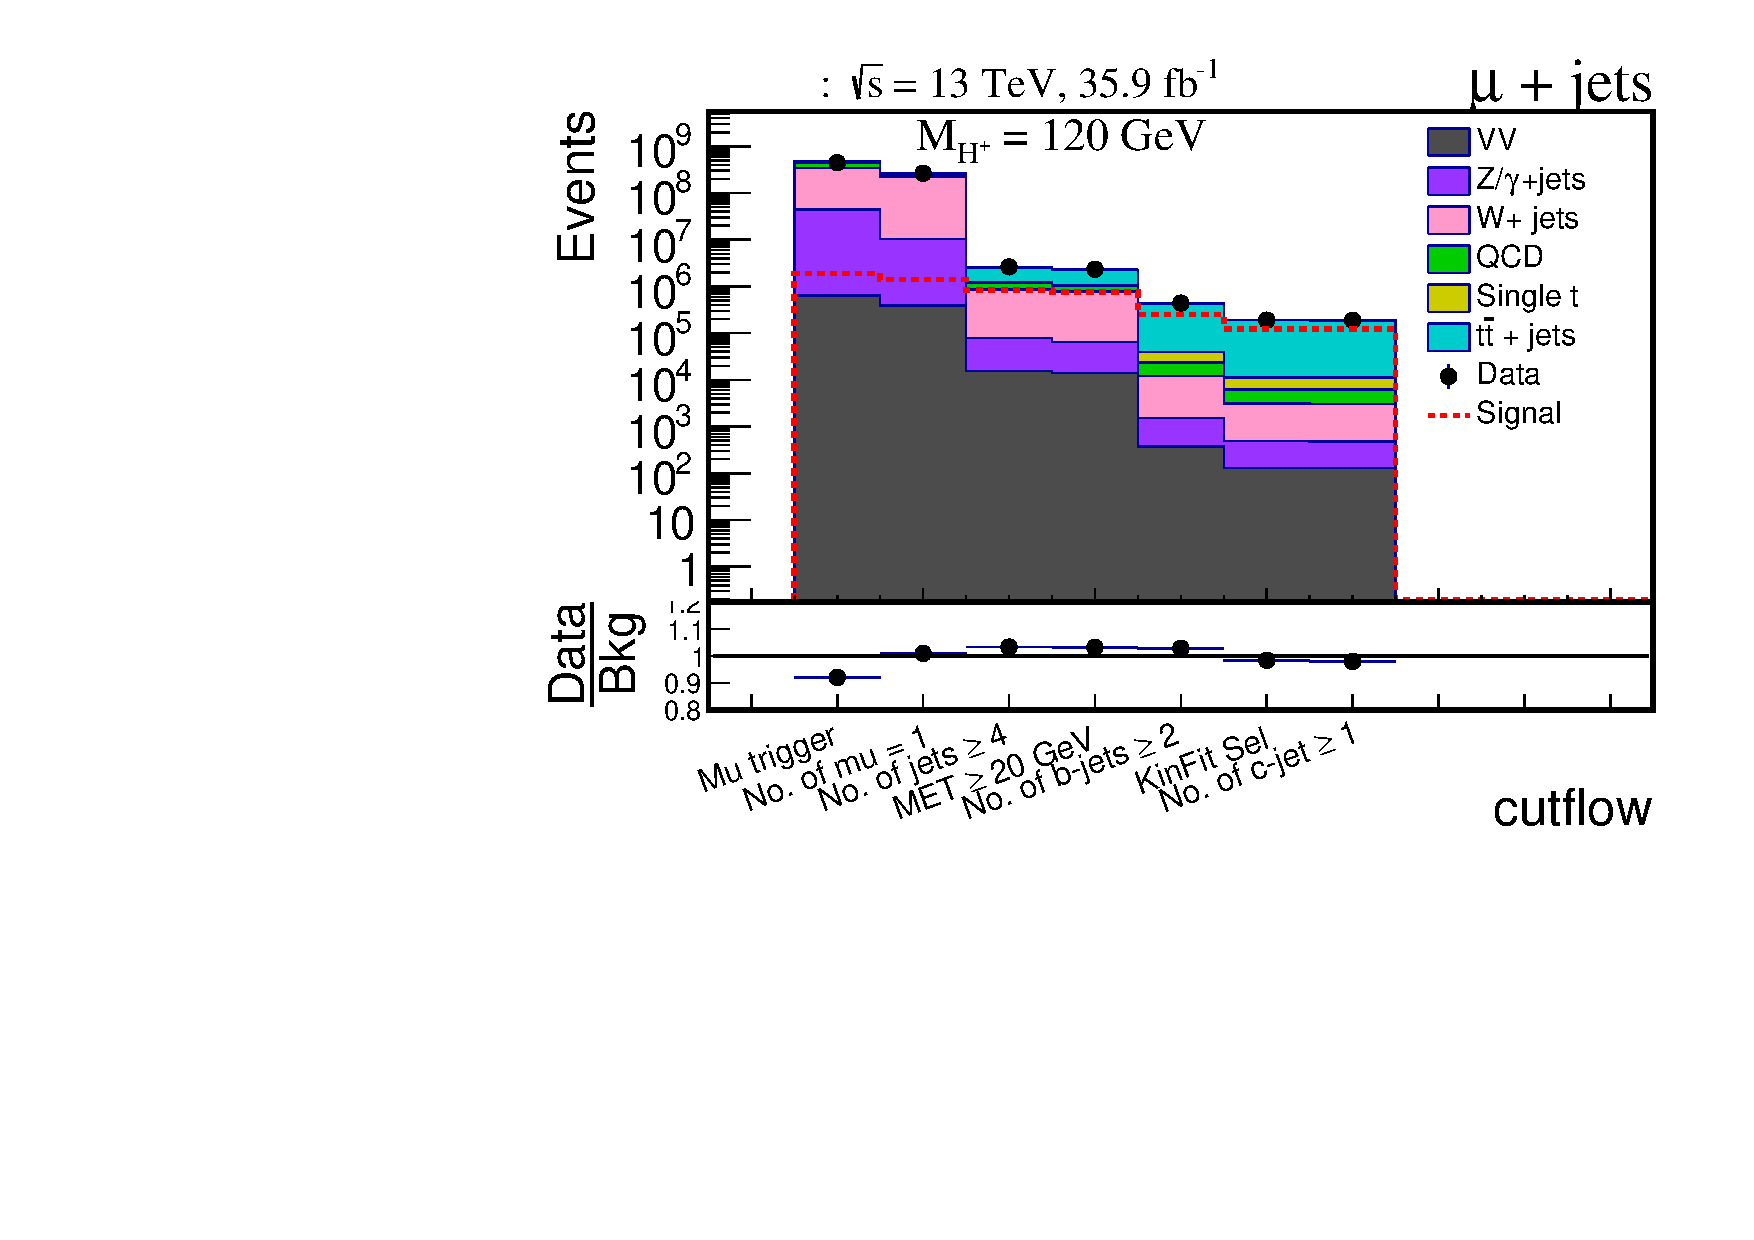
\includegraphics[width=0.45\linewidth]{Image/Muon/cutflow_mu_PG.pdf}}
    \subfigure[With $POWHEG$ \ttjets sample
    \label{subfig:cutflow_ele_PG}]
    {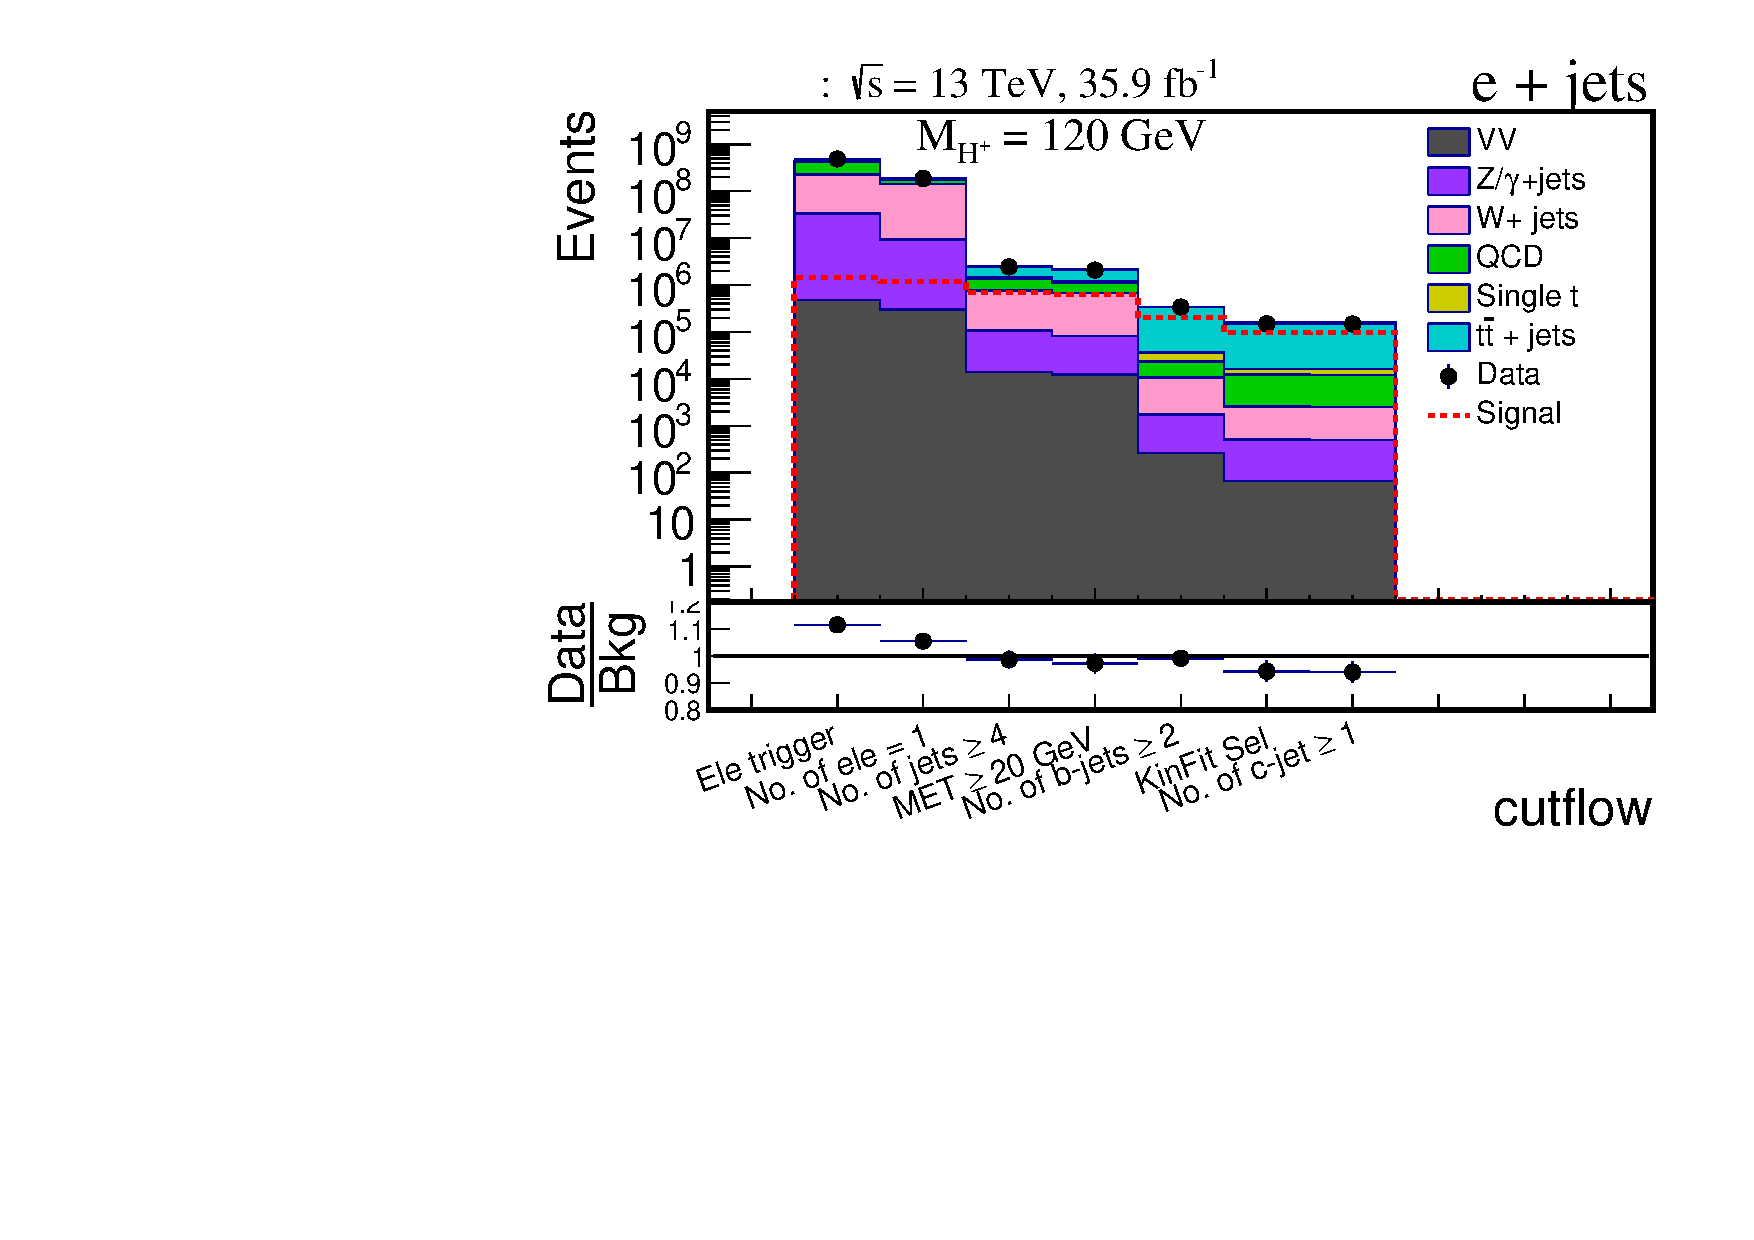
\includegraphics[width=0.45\linewidth]{Image/Electron/cutflow_ele_PG.pdf}}
    \caption{Number of events for MC and data samples after various selection cuts for muon +
    jets and \ejets channel. Number of events differ only after $N_{jets} \geq 4$ cut
    as can be seen from Figure\ref{subfig:cutflow_mu_MG},~\ref{subfig:cutflow_mu_PG} for \mujets
    channel and from Figure\ref{subfig:cutflow_ele_MG},~\ref{subfig:cutflow_ele_PG} for electron + 
    jets channel. From Figure\ref{subfig:cutflow_mu_PG},~\ref{subfig:cutflow_ele_PG}, it can be seen
    that the data, MC has better agreement with $POWHEG$ \ttjets sample. Except for 
    \ttjets, all the other MC samples are same in Figure\ref{subfig:cutflow_mu_MG},
    ~\ref{subfig:cutflow_mu_PG} for \mujets channel and in Figure\ref{subfig:cutflow_ele_MG},
    ~\ref{subfig:cutflow_ele_PG} for \ejets channel. The muon(electron) enriched MC QCD 
    samples as shown in Table~\ref{tab:mcSample} are used for muon(electron) + jets channels.}
    \label{fig:MGvsPG}
\end{figure}
